\section{Particle Physics detectors}

In order to detect a particle it must interact with the material of the detector and transfer energy in some recognisable fashion.
\paragraph{Particle detection occurs via the energy loss of particles through the material they traverse.} In the end, all signals we record are electromagnetic signals. So we can discover charged particles. Neutral particles need to be converted to charged particles to be seen. This happens in an electromagnetic calorimeter with photons $\gamma \to e^+ e^-$, and in hadronic calorimeters via nuclear interactions that create charged pions and protons.

\paragraph{Possibilities}
\begin{itemize}
\item[(i)] EM charged particles $\rightarrow$ Ionisation, Bremsstrahlung$^*$, Cherenkov
\item[(ii)] Hadrons $\rightarrow$ Nuclear interactions$^*$ (equivalent to ones above the involving the strong force)
\item[(iii)] Photons $\rightarrow$ Pair production$^{**}$, Photoelectric effect, Compton effect
\end{itemize}
$^{(*)}$ Cause a shower of particles (see later).\newline
$^{(**)}$ Total energy loss via a single interaction converting into charged particles.\newline
Some examples of what these processes look like:

\begin{center}
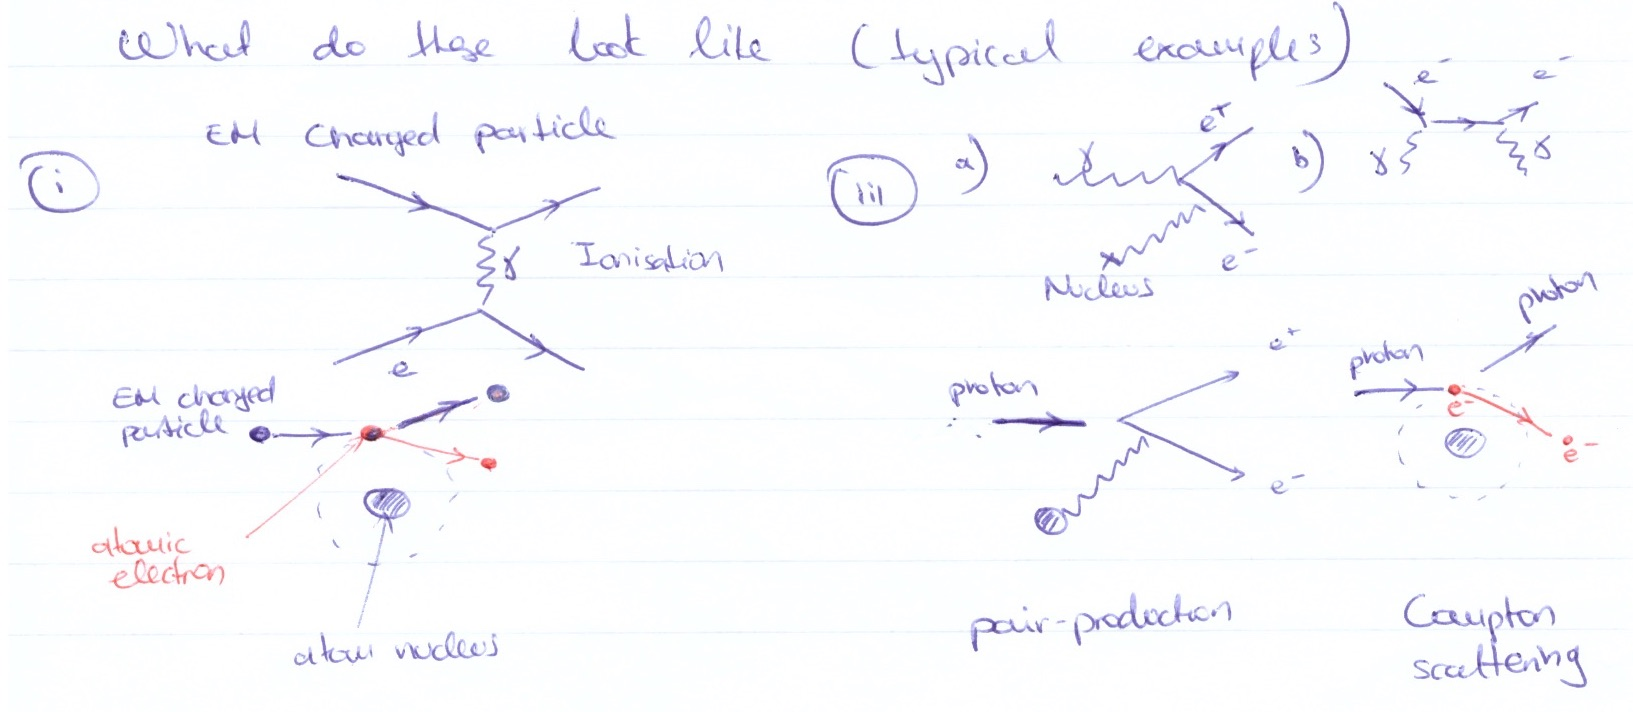
\includegraphics[width=0.95\textwidth]{fig/strongforce/matterinteractions/interactions1.jpg}\newline
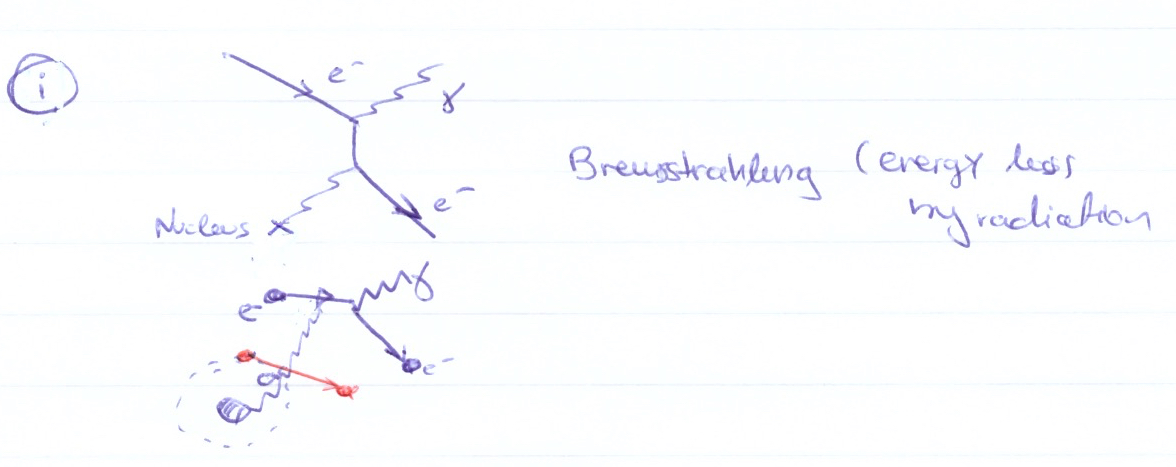
\includegraphics[width=0.8\textwidth]{fig/strongforce/matterinteractions/interactions2.jpg}
\end{center}

A lot more information of this section can be found in Appendix~\ref{sec:interaction_particle_matter} that is not examinable but quite interesting!


\subsection{Putting together a particle physics detector}
\label{sec:detectorSummary}
\begin{center}
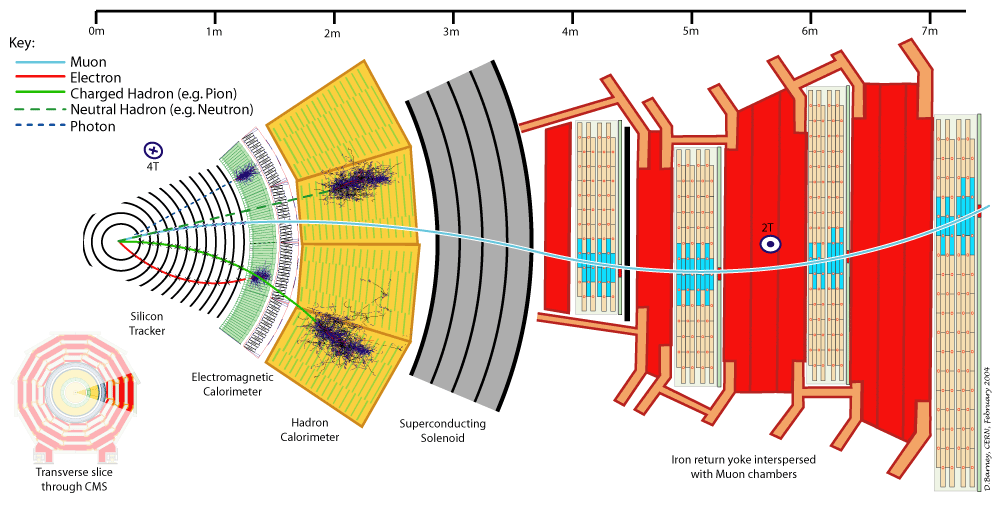
\includegraphics[width=0.95\textwidth]{fig/detector/cms_slice.png}
\end{center}

The inner most part of a detector is typically made up of relatively low radiation and interaction length material aimed at making a precise measurement of the initial collision point and of subsequent decay vertices. This is achieved by reconstructing the trajectories of outcoming charged particles as they deposit energy via ionisation. They are called ``vertex detectors'' and are typically made up of silicon pixel or strip sensors. 

Following the vertex detectors, one finds further detectors aimed at reconstructing the trajectories of charged particles by detecting ionisation energy as the particles traverse through them (``Tracking detectors''). By placing a magnetic field and measuring how the trajectory of the particles bends, we can get an estimate of their momentum.

Past the tracking detectors one can place RICH detectors (e.g at LHCb) aimed at measuring the speed of the particle, and combining with the measurement of the momentum obtain an estimate of the particle's mass and hence its type. One can also place an ECAL after the tracking (and after the RICH systems) to measure the energies of photons and electrons. As hadrons have masses much larger than the electron mass, they will not have an EM shower in the ECAL and will not form a hadronic shower either, as the typical interaction length ($\lambda$) of the ECAL is much too small (ECALs are less dense than HCALs). 

After the ECAL follows the HCAL. In the HCAL hadrons like pions, Kaons and protons will perform a hadronic shower, allowing for the measurement of their energies. Energies of jets of hadrons initiated by quarks and gluons, are measured by combining information from the tracking systems and calorimeters.

Muons are a special case. As $m_\mu\sim m_\pi\gg m_e$ and muons do not undergo strong interactions, they pass through the ECAL and HCAL by simply depositing a minimum amount of ionisation energy. Therefore in order to detect muons, detection systems aimed at measuring deposits of ionisation energy are placed after the HCAL, allowing for both the identification of muons (as mainly muons would reach the outer parts of the detectors) as well as the measurement of the momentum as the muon bends in the magnetic field. Muons are therefore very easy to distinguish from other particles: They are the one charged particle that makes it through all the mass in the calorimeters and survives until the muon detectors. Particle physicists love decays with muons int he final state!

\begin{center}
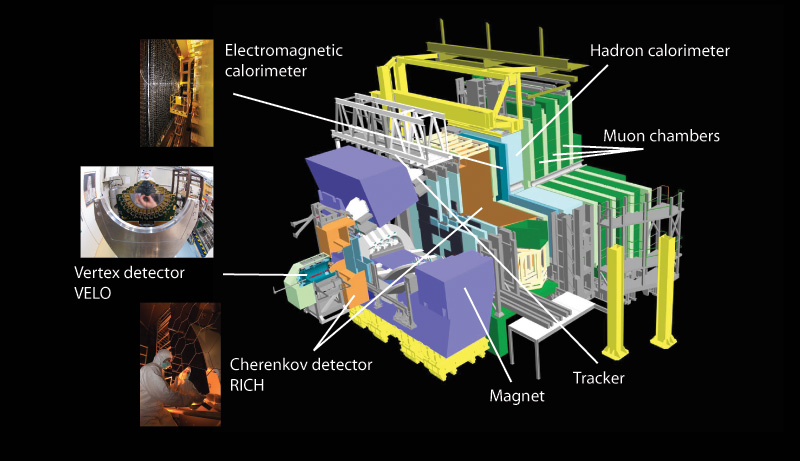
\includegraphics[width=0.95\textwidth]{fig/detector/lhcb_detector.png}
\end{center}
The figure below shows a similar configuration for the LHCb detector.

\subsection{Missing transverse momentum (or energy)}
This has already been discussed in \secref{sec:missingEt}, but is repeated here under a slightly different angle, because it also belongs into the detector section, and because it is important.

In hermetic ($4\pi$) detectors like CMS and ATLAS, particles that only very rarely interact
with matter (such as neutrinos and particles proposed in theories beyond the Standard Model such as Supersymmetry or hypothesised Dark Matter candidate particles) are detected by their absence. What do we mean by that? 

In a $pp$ collision (or any collision) where the protons are primarily only have momentum along the horizontal axis, the total initial momentum transverse to the direction of the protons is zero. Therefore after the collision, momentum should be conserved and thus the total momentum obtained by summing over all the outcoming particles from the collision (this is why detectors like CMS that completely surround the collision are important), transverse to the direction of the protons ie 
\[{\rm Missing\,\,Transverse\,\,Momentum}=-\sum_{\rm i=1..N_{\rm particles}} p_{T}^{i}\]
should add up to zero. If it does not then it means that particles where produced which did not interact with the detector. Such particles could have been known neutrinos or, depending on the amount of missing energy, momentum could be Dark Matter candidates.
The figure below, is a $t\bar{t}$ event from CMS where each of the $t$-quarks decay to a $b$ quark (which forms a jet) and a $W$ boson which subsequently decays to a $\mu$ and a $\nu_{\mu}$. The sum of the momenta that the two $\nu$'s carry (one from the $t$ and another from the $\bar{t}$) is inferred by the mis-balance of momentum (or equivalently energy) in the transverse plane and is denoted by the purple arrow labelled $\cancel{\rm E_{T}}$.
\begin{center}
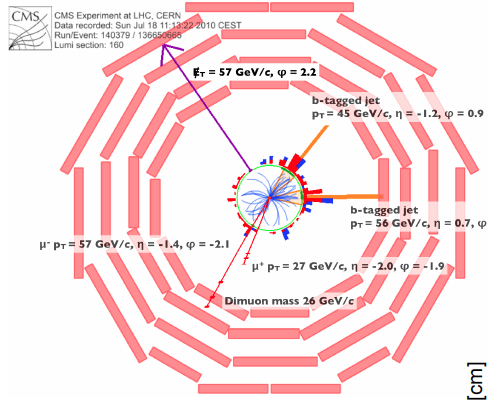
\includegraphics[width=0.75\textwidth]{fig/detector/met_cms.png}
\end{center}

An example of a process that makes use of all detector components of the detector is the production of top quarks at the LHC. Top quarks have a very short lifetime. 
\[\tau_{t}=5\times 10^{-25}s\]
However the time at which QCD confinement acts (ie the time scale in which a quark binds into a hadron) can be calculated as follows:

QCD confinement takes place at an energy scale 
\[
\Lambda_{QCD}=200~{\rm MeV}.
\]
We can convert this energy scale into a timescale using 
\[
\hbar c=200~{\rm MeV~fm}
\]
(this is something you should commit to memory as it is a very useful quantity for a particle physicist).
Therefore
\[
\tau_{QCD}=\hbar c\times\frac{1}{c\Lambda_{QCD}}=3\times 10^{-24}s
\]
As $\tau_{QCD}<\tau_{t}$, the top quark decays before it has a change to form a bound state! 

Due to the CKM elements involved, the top quark predominantly decays to a b-quark 
\[t\rightarrow b W\]
where the $b$-quark will in turn produce a jet of particles which contains at least one hadron with a $b$-quark. This so called $b$-jet can be identified both through the stream of hadrons producing tracks in the tracking system and energy depositions in the calorimeters, as well as through the displaced vertex formed by the decay products of the $B$-hadron.
The $W$ will in turn decay into a lepton or a pair of quarks. In the case that the $W$ decays to a lepton and a neutrino, the neutrino escapes the detector and its existence is inferred through missing transverse energy.
